% !TeX spellcheck = <none>
%%%%%%%%%%%%%%%%%%%%%%% file template.tex %%%%%%%%%%%%%%%%%%%%%%%%%
%
% This is a general template file for the LaTeX package SVJour3
% for Springer journals.          Springer Heidelberg 2010/09/16
%
% Copy it to a new file with a new name and use it as the basis
% for your article. Delete % signs as needed.
%
% This template includes a few options for different layouts and
% content for various journals. Please consult a previous issue of
% your journal as needed.
%
%%%%%%%%%%%%%%%%%%%%%%%%%%%%%%%%%%%%%%%%%%%%%%%%%%%%%%%%%%%%%%%%%%%
%
% First comes an example EPS file -- just ignore it and
% proceed on the \documentclass line
% your LaTeX will extract the file if required
\begin{filecontents*}{example.eps}
%!PS-Adobe-3.0 EPSF-3.0
%%BoundingBox: 19 19 221 221
%%CreationDate: Mon Sep 29 1997
%%Creator: programmed by hand (JK)
%%EndComments
gsave
newpath
  20 20 moveto
  20 220 lineto
  220 220 lineto
  220 20 lineto
closepath
2 setlinewidth
gsave
  .4 setgray fill
grestore
stroke
grestore
\end{filecontents*}
%
\RequirePackage{fix-cm}
%
%\documentclass{svjour3}                     % onecolumn (standard format)
%\documentclass[smallcondensed]{svjour3}     % onecolumn (ditto)
\documentclass[smallextended]{svjour3}       % onecolumn (second format)
%\documentclass[twocolumn]{svjour3}          % twocolumn
%
\smartqed  % flush right qed marks, e.g. at end of proof
%
\usepackage[utf8]{inputenc}
\usepackage[english]{babel}
%\usepackage{natbib}
%\usepackage[round, sort]{natbib}
\usepackage{amsmath}
\usepackage{amsfonts}
\usepackage{amssymb}
\usepackage{graphicx}
\usepackage{mathtools}
\usepackage[left=2cm,right=2cm,top=2cm,bottom=2cm]{geometry}
\usepackage{gensymb} 
\usepackage{float}
% \usepackage{notoccite}
 %\usepackage{natbib}
%\bibliographystyle{abbrvnat}
%\setcitestyle{authoryear,open={((},close={))}}
%\usepackage[style=authoryear]{biblatex}
%\addbibresource{<your-bib-file.bib>} % note the .bib is required

	%\printbibliography






%\usepackage{graphicx}
%\usepackage[utf8]{inputenc}
%\usepackage[english]{babel}
%\usepackage[
%backend=biber,
%style=alphabetic,
%citestyle=authoryear
%]{biblatex}
% \usepackage{mathptmx}      % use Times fonts if available on your TeX system
%
% insert here the call for the packages your document requires
%\usepackage{latexsym}
% etc.
% please place your own definitions here and don't use \def but
% \newcommand{}{}
%
% Insert the name of "your journal" with
% \journalname{myjournal}
%

\begin{document}

\title{Insect Demography: ***%\thanks{Grants or other notes
%about the article that should go on the front page should be
%placed here. General acknowledgments should be placed at the end of the article.}
}
%\subtitle{Do you have a subtitle?\\ If so, write it here}

%\titlerunning{Short form of title}        % if too long for running head

\author{Elisha B. Are \and
  Jonathan Dushoff \and John W. Hargrove %etc.
}

%\authorrunning{Short form of author list} % if too long for running head

\institute{Elisha B. Are \at
              Centre of Excellence in Epidemiological Modelling and Analysis (SACEMA), University of Stellenbosch, Stellenbosch, South Africa. \\
              Tel.: +27653249688\
              \email{elishaare@sun.ac.za}           %  \\
%             \emph{Present address:} of F. Author  %  if needed
           \and
           Jonathan Dushoff \at
            Department of Biology, McMaster University, Hamilton, Ontario, Canada
             \and
             John W. Hargrove \at
            Centre of Excellence in Epidemiological Modelling and Analysis (SACEMA), University of Stellenbosch, Stellenbosch, South Africa. 
             }

\date{Received: date / Accepted: date}
% The correct dates will be entered by the editor


\maketitle

\begin{abstract}
 .\vskip 0.2cm	
As insect populations decline, due to climate change and other environmental disruptions, there has been an increased interest in understanding extinction probabilities. Generally, the life cycle of insects occurs in well-defined stages: when counting insects, questions naturally arise about which stage to count and the appropriate point to start counting. 
Using tsetse flies (vectors of the trypanosomiasis) as a case study, we develop a model that works for different counting points in the life cycle of a fly. We analyse reproductive numbers and extinction probabilities, and show that several previous models used for estimating extinction probabilities for tsetse populations are special cases of the current model.  
We establish that the reproduction number is the same for different counting points, but that the extinction probability is different for each counting point. We demonstrate, and provide a biological explanation for, a simple relationship between extinction probabilities for the different counting points, based on the probability of recruitment between stages.
These results offer insights into insect population dynamics and provide tools that will help with more detailed models of insect populations. Demographic studies of insects should be clear about life stages and counting points. 
\keywords{Extinction probability \and Insect Demography \and Tseste ({\it Glossina} spp) \and Geometric Distribution}
% \PACS{PACS code1 \and PACS code2 \and more}
\subclass{60D05  \and 92B05 \and 60G50 }
\end{abstract}

\section{Introduction}
\label{intro}
 
Insects play key ecological roles, both positive and negative, for the health of plants and animals, including humans, and for the environment in general \cite{Ollerton2011,Ockinger2007}.    Many are important vectors of plant and animal diseases, often of public health importance \cite{Tobias2016,Wamwiri2016,Beier1998}, others are beneficial in, for example, pollination, a few serves as source of protein for massive numbers of species of animals including humans \cite{Ramos-Elorduy1997}. Biologists are accordingly interested in insect population persistence for various reasons. On one hand, conservationists are concerned about the ecological implications of extinction of insect populations, whereas vector biologists may be interested in the control/elimination of insect vectors \cite{Burt2015,Shaw2013,Hocking1963}.  In whichever way we look at things, the study of insect population dynamics is clearly an important area of research. \\


There have been claims, in the literature, that various insect populations are exhibiting catastrophic declines in numbers in different parts of the world \cite{Conrad2002,Potts2010,Ilyinykh2011,VanSwaay2013,Lister2018}. Hallmann et al \cite{Hallmann2017} reported an alarming decline of 75\% in the biomass of flying insects over a 27 year period, in 63 protected areas of Germany. Similar findings of major decline have been reported across the globe \cite{Habel2015,Pelton2019}. For instance, there was a decline of 50\% in the population abundance of European grassland butteries between 1990 and 2011 \cite{VanSwaay2013}, and it has been reported that tsetse populations have been declining in the Zambezi valley of Zimbabwe \cite{Lord2018}. If the magnitude of the declines is as serious as reported, the earth may soon witness extinction of several insect species.\\


  
Since insects are cold blooded, their body temperature is basically determined by the ambient temperature that they are experiencing – making them vulnerable, for example, to the effects of global warming. There is therefore a growing concern about how increases in global temperature, and other environmental disruptions, will impact insect populations. In recent years, questions involving extinction of several insect populations are now being asked more frequently \cite{Nilsson2017}. Accordingly, there is a need to continue to improve the accuracy of our prediction of the probability of extinction events in insects – and indeed other animals and plants. \\


The life history of insects occurs in well-defined stages and the possibility therefore exists of counting insect population according to the numbers of different stages. One may choose to count the numbers in a particular juvenile stage or, alternatively, at some more mature stages. The question then arises as to whether it makes any difference which developmental stage is counted when one is calculating – for example – the probability that an insect population goes extinct.  We investigate this problem, using populations of tsetse (Glossina spp) as an illustrative example. Tsetse are vectors of trypanosomiasis \cite{Wamwiri2016,Kioy2004}; a deadly disease called African sleeping sickness in humans and nagana in livestock \cite{Kioy2004}. The life cycle of the fly involves four distinct stages; namely, larva, pupa, newly emerged adult, and mature adult – the last stage in females being defined as those flies that are larvipositing \cite{Ackley2017a}. We pose the question of whether it matters which stage we count. How would accounting for different insect life stages affect our calculation of the probability that an insect population will persist under various circumstances? \\


Several workers have developed varieties of mathematical models to explain different phenomena in insect population dynamics, but are generally not clear about which developmental stage(s) are being counted \cite{Ylioja1999,Artzrouni2003,Hargrove2005a,Adams2005,Barclay2011d,Peck2012a,Lin2015,Kajunguri2019}.  As far as we are aware, no published work in the literature has explicitly considered the implication of counting insects at different stages for the estimation of extinction probabilities for insect populations. Hargrove \cite{Hargrove2005a} developed and analysed a branching process model to derive expressions for extinction probabilities, times to extinction, reproduction number and variance for closed populations of tsetse. The results reported in \cite{Hargrove2005a} agree with published work in the literature on tsetse vital rates, and showed that quite small increases in mortality rates,  could drive any population of tsetse to extinction. Kajunguri et al \cite{Kajunguri2019} improved on some of the assumptions in \cite{Hargrove2005a}, specifically, the assumption about the relationship between the male to female sex ratio of pupae produced and how this affects extinction probabilities. They also provided mathematical proofs of the results presented in \cite{Hargrove2005a}. The work has been extended to provide estimates of extinction probabilities, growth rates, reproduction number and times to extinction as a function of the temperature that the flies are experiencing \cite{Are2019}. \\



In the above studies, the modelling framework was built on the assumption that the pioneer population starts with one or more newly emerged adult female tsetse. In the current study, by contrast, we  generalise the approach – allowing that the population can start with either larvae/pupae, or newly emerged adults, or mature/larvipositing females and we compare the outcomes for each of these scenarios. We establish a relationship between the extinction probabilities for tsetse populations where the pioneer population consists only of individuals at one of the three life stages defined above. We discuss, in detail, the implications of our results to tsetse population persistence, particularly in the context of tsetse control/eradication exercises. \\


 

\subsection{\bf Brief description of tsetse life cycle}

Tsetse typically mate once in their life-time: the sperm deposited by a fertile male, during mating, is sufficient for the female to fertilize all subsequent eggs throughout her life. A female fly produces, typically every 9-11 days, a single larva, which may weigh as much or even more than she does herself.  The larva borrows into the soil and pupates within minutes. The pupal period lasts 30 - 50 days \cite{PhelpsR.J.&Burrows}, depending on soil temperature. After the pupal period, an immature adult emerges. It takes 7-9 days, depending on temperature, for the newly emerged adults to attain full maturation – approaches which involves the development of a mature thoracic musculature and fat reserves. During this period females are typically inseminated by a male tsetse, and virtually all will have ovulated by the age of 10 days \cite{Hargrove2012c}. The fully developed adult typically larviposits every 9-11 days afterwards \cite{Hargrove2019}. Unlike other insects, say mosquitoes, which can produce up to 100 eggs at a time \cite{Clemons2010}, tsetse produce a single offspring at a time, consequently, their birth rate is relatively low. 


%\section{Section title}
%\label{sec:1}
%Text with citations \cite{RefB} and \cite{RefJ}.
%\subsection{Subsection title}
%\label{sec:2}
%as required. Don't forget to give each section
%and subsection a unique label (see Sect.~\ref{sec:1}).
%\paragraph{Paragraph headings} Use paragraph headings as needed.
%\begin{equation}
%a^2+b^2=c^2
%\end{equation}

% For one-column wide figures use

\section{Mathematical Models}
In this section, we develop three models, each representing different counting stage in the life history of tsetse. This models account for the three stages of tsetse life cycle. We acknowledge that  counting point may differ from  starting point, however for simplicity sake, we assume that the count point is the same as the starting point. The models are developed based on the schematic presented in Figure \ref{fig:tsetseflowchat3}, with the following variables and parameter descriptions:

\begin{itemize}
\item[•] $p_c$: probability a newly deposited larva survives to emerge as a young female adult
\item[•] $p_o$: probability a newly emerged adult survives to reach larviposition loop
\item[•] $p_{l}$: probability of surviving a larviposition loop
\item[•] $P_{d}$: larva deposited
\item[•] $A_{e}$: young adult emerges
\item[•] $A_{o}$: adult enters larviposition loop 
\end{itemize}
\begin{figure}[hbt!]
	\centering
	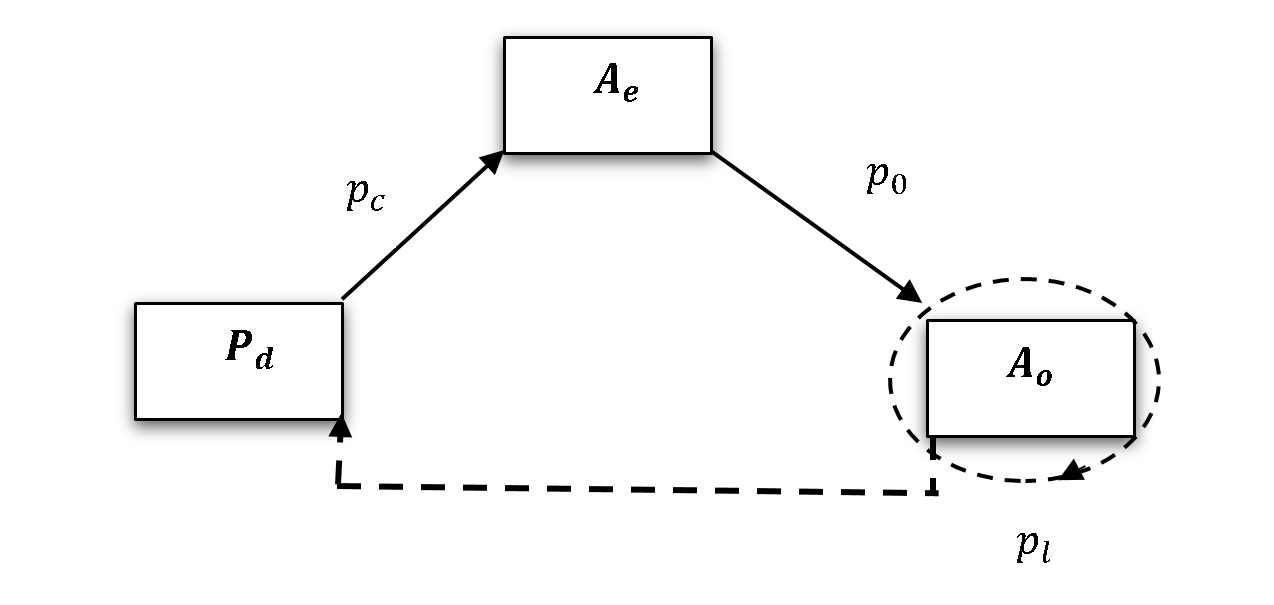
\includegraphics[width=0.7\linewidth]{Tsetseflowchat3}
	\caption{A schematic diagram for counting tsetse}
	\label{fig:tsetseflowchat3}
\end{figure}

For each counting stage we derive an offspring probability distribution, and analyse the reproductive number and extinction probability.    

\subsection{\bf Model 1: Counting point - Larva}

Here we develop a distribution function for the probability that a newly deposited larva develops to the stage of larviposition and produces exactly $k$ surviving female larvae in her life time. A deposited larva survives then emerge as a young female adult with probability $p_{c}$, reaches the larvipostion loop with probability $p_o$, and completes one successful larviposition cycle with probability $p_{l}$. The probability that the female larva reaches the larviposition loop and produces exactly $k$ larvae before it dies is:

\begin{equation}
\label{larvadistribution}
p_{k}^{d} = p_{c}p_{o}(\frac{p_{l}}{1-p_{l} + p_{l}})^{k}(1-p_{l})= p_{c}p_{o}p_{l}^{k}(1-p_{l}), k =0,1,2,...
\end{equation} 
Equation (\ref{larvadistribution}) can be obtained either by following the proceedure presented in \cite{Kajunguri2019} or by induction.\\

The generating function for  $p_{k}^{d}$ is:

\begin{equation}
\label{GenFunction}
 G(s) = \sum_{k=0}^{\infty} p_{k}^{d}s^{k},  
\end{equation}
where $ 0\leq s \leq 1.$ \\

Equation (\ref{GenFunction}) can be used to obtain the reproduction number and extinction probabilities for tsetse populations. 

\subsubsection{\bf Reproduction number $R_{d}$}

The reproduction number $R_{d}$ is the expected number of larvae that a newly deposited female larva is expected to produce in her lifetime. $R_{d}$ is defined as $G'(1)$ (the first derivative of $G(s)$ w.r.t $s$), and is given by:

\begin{equation}
\label{larvareproductiveNum}
R_{d} = G'(1) = \frac{p_{c}p_{o}p_{l}}{1-p_{l}}.
\end{equation}  



\subsubsection{\bf Extinction probability  $q_{d}$}

To calculate the extinction probability for a tsetse population starting with a single newly deposited larva, we rewrite $p_{k}^{d}$ in the form $bc^{k-1}$ with $k =1,2,...$ and $b,c > 0$ (this is to allow us to follow the proceedure used by Harris \cite{Harris1965} to calculate the extinction probability). It follows from  \cite{Harris1965}, that the generating function is a fractional linear type. The extinction probability is the smaller root of $G(s)=s$, given by: 

\begin{equation}
\label{harrisresult}
q = \frac{1 - b -c}{c(1-c)},
\end{equation}
if we set $q = s$ and  $b, c < 1$.\\

The proof of equation (\ref{harrisresult}) follows from the fractional linear generating function associated with $bc^{k-1}$ \cite{Harris1965}. \\

After rewriting $p_{k}^{d}$ in the form $bc^{k-1}$, we have  $$b = p_{c}p_{o}p_{l}(1-p_{l})$$ and $$c = p_{l}$$ 

The probability of extinction for a population starting with a newly deposited  female larva is obtained by substituting the values of $b$ and $c$ into equation (\ref{harrisresult}). After some algebraic simplifications we have:

\begin{equation}
\label{extictionLarva}
q_{d} = \frac{1-p_{c}p_{o}p_{l}}{p_{l}}, p_{l} \neq 0.
\end{equation}



\subsection{\bf Model 2: Counting point - Newly emerged adult}

In similar fashion to the development of model 1, we obtain a distribution function for the probability that a newly emerged female adult tsetse reaches the larviposition loop and produces exactly $k$ surviving young female adults.
A newly emerged adult fly survives to the larvipositing stage  with probability $p_{o}$  and  completes one successful larviposition cycle with probability $p_{l}$. Our interest is in the number of deposited larvae that emerge as young adults. The probability that a newly emerged female tsetse produces exactly $k$ surviving newly emerged female adults, before dying, is: 

\begin{equation}
\label{distributionYoungadult}
p_{k}^{e} = p_{o}(\frac{p_{c}p_{l}}{p_{c}p_{l} + 1 - p_{l}} )^{k}\frac{1-p_{l}}{p_{c}p_{l} + 1 - p_{l}}, k =0,1,2,...
\end{equation}      

\subsubsection{\bf Reproduction number $R_{e}$}

The number of young adults a young adult female is expected to produce in her life time is obtained by following the same procedure used for equation (\ref{larvareproductiveNum}).

\begin{equation}
\label{YoungAdulreproductiveNum}
R_{e} = G'(1) = \frac{p_{c}p_{o}p_{l}}{1-p_{l}},
\end{equation}  
where $G(s) = \sum_{k=0}^{\infty} p_{k}^{e}s^{k}  $, $0\leq s \leq 1$, is the generating function for $p_{k}^{e}$.

\subsubsection{\bf Extinction probability  $q_{e}$}

The probability of extinction for a population of tsetse starting with a single newly emerged female fly is obtained by rewriting equation (\ref{distributionYoungadult}) in the form $bc^{k-1}$, where,

$$ b = \frac{p_{o}p_{c}p_{l}(1-p_{l})}{(p_{c}p_{l} + 1 - p_{l})^{2}} $$ and

$$ c = \frac{p_{c}p_{l}}{p_{c}p_{l} + 1 - p_{l}} , $$ 

Inserting $b$ and $c$ into equation (\ref{harrisresult}) gives:

\begin{equation}
\label{extinctionYoungadult}
q_{e} = \frac{1- p_{l}(1 -p_{c}(1- p_{o}))}{p_{l}p_{c}}
\end{equation}


\subsection{\bf Model 3: Counting point - Larvipositing adult}

The distribution function for the probability that a larvipositing  adult produces exactly $k$ surviving larvipositing adults is obtained as follows: a larvipositing female adult completes  a successful  larviposition loop with probability $p_{l}$ and each larva she deposits develops to emerge as a female adult with probability $p_{c}$, and reaches the larviposition stage with probability $p_{o}$.  The probability that a larvipositing tsetse produces exactly $k$ surviving larvipositing female, before it dies, is thus:

\begin{equation}
\label{OvulatingAdultdistribution}
p_{k}^{o} = (\frac{p_{o}p_{c}p_{l}}{p_{o}p_{c}p_{l} + 1 - p_{l}})^{k}\frac{1 - p_{l}}{p_{o}p_{c}p_{l} + 1 - p_{l}}, k =0,1,2,...
\end{equation}




\subsubsection{\bf Reproduction number $R_{o}$}
The reproduction number for tsetse population, starting with a single larvipositing female, is obtained by following the procedure decribed earlier. 
\begin{equation}
\label{OvulatingadultreproductiveNum}
R_{o} = G'(1) = \frac{p_{c}p_{o}p_{l}}{1-p_{l}},
\end{equation}  
where $G(s) = \sum_{k=0}^{\infty} p_{k}^{o}s^{k}  $, $0\leq s \leq 1$, is the generating function for $p_{k}^{o}$.

\subsubsection{\bf Extinction probability  $q_{o}$}

The reproduction number for a tsetse population, starting with a single larviposting female in the initail population, is obtained by writing  (\ref{OvulatingAdultdistribution}) in terms of  $R_{o}$. This yields:

\begin{equation}
\label{OvulatingAdultExtinct}
p_{k}^{o} = (\frac{R_{o}}{R_{o} + 1})^k\frac{1}{R_{o} + 1}, k =0,1,2,...
\end{equation}
Notice that equation (\ref{OvulatingAdultExtinct}) forms a geometric distribution, with generating function  $$G(s) = \frac{p}{1-s(1-p)}, $$ where $0\leq s \leq 1$. Writing this in terms of $R_o$, and setting $G(s)=s$, gives a quadratic :

\begin{equation}
\label{QuardAdultExtinct}
s =s^2\frac{R_{o}}{R_{o} + 1} + \frac{1}{R_{o} + 1} ,
\end{equation} 

Factoring equation (\ref{QuardAdultExtinct}), yields:
 $$(R_os-1)(s-1) = 0$$ $\implies s=1/R_o$ or $s=1$. Setting $s=q_o$,  the probabalilty of extinction for a population of tsetse, starting with a single larvipositing adult, gives: 


\begin{equation}
\label{extinctionYoungadult}
q_{o} = \frac{1-p_{l}}{p_{c}p_{o}p_{l}} = \frac{1}{R_{o}},
\end{equation}
where $R_o > 1$.

\section{\bf Relationship between $q_{o}$, $q_{e}$ and $q_{d}$}

In this section, we establish a relationship between extinction probabilities for tsetse populations, starting with different life stages in the initial population. 

\subsubsection*{Theorem I}
Suppose $q_{d}$, $q_{e}$ and $q_{o}$ are as defined earlier. Then,  given that $R_{o}>1$ the following inequality holds:
\begin{equation}
\label{Aretsetsetheorem}
q_{o}\leq q_{e} \leq q_{d}
\end{equation}

\subsubsection{Proof of Theorem I}
\subsubsection{Part A}
If  $q_{e} < q_{o}$, %and that $R_{o} > 1$ (Supercritical case) \\
$$ \frac{1- p_{l}(1 -p_{c}(1- p_{o}))}{p_{l}p_{c}} < \frac{1-p_{l}}{p_{c}p_{o}p_{l}} = \frac{1}{R_{o}}, $$

\begin{equation}
\label{contradiction1}
\implies       \frac{p_{o}}{R_{o}} - p_{o} + 1 < \frac{1}{R_{o}}. 
\end{equation}

From triangular inequality $( |a + b| \leq |a| + |b|)$ and  that $R_{o} > 1$, equation (\ref{contradiction1}) yields a contradiction. Hence, $q_{o} \leq q_{e}$. 
\subsubsection{Part B}
If $q_{d} < q_{e}$,

$$  \frac{1-p_{c}p_{o}p_{l}}{p_{l}}  < \frac{1- p_{l}(1 -p_{c}(1- p_{o}))}{p_{l}p_{c}},  $$

\begin{equation}
\label{contradiction2}
\implies  \frac{1}{p_{l}} - p_{c}p_{o} - 1 <     \frac{p_{o}}{R_{o}} - p_{o}.
\end{equation}
Using the same assumption as in Part A, equation (\ref{contradiction2}) yields a contradiction. Hence, $q_{e} \leq q_{d}$. Since $"\leq"$ is transitive on ${\Bbb R}$, the proof is complete.

\subsubsection*{\bf Remark I}
We obtained the same reproduction number explicitly for different counting points. This is clear from  $R_{d} = R_{o}=R_{o}$ (see equations (\ref{larvareproductiveNum}), (\ref{YoungAdulreproductiveNum}) and (\ref{OvulatingadultreproductiveNum})), without any extra assumption. However, to recover the same extinction probabilities for the three different counting points, extra assumptions are required. The extinction probability for {\bf Model 2} is the same as the extinction probability for {\bf Model 3} ($q_{e} =q_{o}$), if $p_{o} = 1$, (corresponding to not counting flies until they are in the ovulation cycle). Moreover, the extinction probability for the three models are the same if we add an extra assumption that $p_{c} =p_{o} = 1$, corresponding to not counting larvae and young adults until they reach the ovulation cycle. \\


\section{\bf A unifying approach to estimating extinction probabilities for tsetse population}

We present here, a general model that works for estimating extinction probabilities, reproduction number e.t.c.   for all counting points. Although tsetse populations are used as an illustrative example, the results are valid for other insect populations, given that their life cycle exists in distinct stages. 


\subsection{\bf Model 4}
Suppose $\hat{p_c}$ is the probability of reaching the "count point" from birth, and $\hat{p_o}$ the
probability of reaching larviposition loop from the "count point". The general offspring distribution function is: 

%Suppose  $A_{x}$ and $A_{y}$ are arbitrary starting and  counting points, respectively. Let $p_{x}$ be the probability of reaching %the ovulation loop from the starting point $A_{x}$; and $p_{y}$ the probability a deposited larva reaches the counting point %$A_{y}$. The probability distribution function is derived to be: 

\begin{equation}
\label{Unifydistfunction} 
p(k) = \hat{p_o}(\frac{p_{l}\hat{p_c}}{p_{l}\hat{p_c}+1-p_{l}})^{k}\frac{1-p_{l}}{p_{l}\hat{p_c}+1-p_{l}},  k =0,1,2,...
\end{equation} 
where $p_{l}$ retains its initial definition. 

\subsubsection{\bf Reproduction number $R_{co}$}
The expected number of offspring produced by an individual for any counting point is obtained as:  
\begin{equation}
\label{UnifyingReproductionNumber}
R_{co} = G'(1) = \frac{\hat{p_c}\hat{p_o}p_{l}}{1-p_{l}},
\end{equation}  

where $G(s)$ is the probability generating function of (\ref{Unifydistfunction}).

\subsubsection{\bf Extinction probability $q_{co}$}
Here we obtain a general expression for extinction probability for tsetse population, for any counting point/stage.  First,  we write equation (\ref{UnifyingReproductionNumber}) in the form $bc^{k-1}$, we then have:
$$ b = \frac{\hat{p_c}\hat{p_o}p_{l}(1-p_{l})}{(\hat{p_c}p_{l} + 1 - p_{l})^2}, $$
and 
$$ c = \frac{\hat{p_c}p_{l}}{(\hat{p_c}p_{l} + 1 - p_{l})}. $$


By substituting for the values of  $b$ and $c$ in equation (\ref{harrisresult}), and simplifying, we obtained the extinction probability for a tsetse population, given any counting point, as:

\begin{equation}
\label{UnifyingextinctionProb}	
q_{co} = \frac{1-p_{l}(1-\hat{p_c}(1-\hat{p_o}))}{\hat{p_c}p_{l}} 
\end{equation}  

\subsubsection{\bf Proposition I}

It is easily verifiable that models 1, 2 and 3 are special cases of model 4. 

\subsubsection*{Proof}

\subsubsection*{Case I}
For model 1, suppose the inital population consists of a single larva, and  set the larval stage as the "count point", the probability that the larva reaches the counting point from birth is $\hat{p_c}=1$ and the probability of reaching the larviposition loop from the "count point" is $\hat{p_o} = p_{o}p_{c}$. Substituting for $\hat{p_c}$ and $\hat{p_o}$ in equation (\ref{Unifydistfunction}) and equation (\ref{UnifyingextinctionProb}), yields Model 1 (equation (\ref{larvadistribution})), with extinction probability:

 $$q_{\hat{p_o}=p_{o}p_{c},\hat{p_c}=1} = \frac{1-p_{c}p_{o}p_{l}}{p_{l}}.$$
Where $p_c$ and $p_o$ retain their definition. Notice that $q_{\hat{p_o}}$ is identical to $q_{d}$.  \\


\subsubsection*{Case II}
Secondly, for model 2, suppose the counting point is the newly emmerged adult female tsetse, the probability that it reaches the larviposition stage is $\hat{p_o} = p_{o}$, the probability of reaching the counting point from birth is $\hat{p_c}= p_{c}$. Substituting for $\hat{p_o}$ and $\hat{p_c}$ in equations (\ref{Unifydistfunction}) and (\ref{UnifyingextinctionProb}) gives Model 2 (see equation (\ref{distributionYoungadult})), with extinction probability: 

$$q_{\hat{p_c}=p_{c},\hat{p_o}=p_{o}} = \frac{1- p_{l}(1 - p_{c}(1- p_{o}))}{p_{l}p_{c}}. $$

This is the same as $q_{e}$

\subsubsection*{Case III}
Model 3 can be derived from equation (\ref{Unifydistfunction}). Suppose the counting point is females that are already in the larviposition loop, $\hat{p_o}=1$, and $\hat{p_c}=p_{o}p_{c}$. Substituting these in equations (\ref{Unifydistfunction}) and (\ref{UnifyingextinctionProb}), yields Model 3, with extinction probability:  

$$q_{\hat{p_o}=1,\hat{p_c}=p_{c}p_{o}} = \frac{1-p_{l}}{p_{c}p_{o}p_{l}},$$ 
which is identical to $q_{o}.$
\subsubsection*{\bf Remark II}
When the inital population consists of $N$ larvae, $N$ newly emerged adults or $N$ larviposing adults, repectively, assuming that for each population, the reproduction and survival processes are independent, extinction probabilites for each each counting stage will be raised to power $N$. That is, the extinction probability will be $q_d^N$, $q_e^N$ and $q_o^N$, repectively.  


\subsection{Extinction probability for  populations starting with individuals at different life stages}
 Extinction probability for a population consisting of individuals at different life stages in the pioneer population, can be estimated  from equations (\ref{extictionLarva}), (\ref{extinctionYoungadult}) and (\ref{OvulatingAdultExtinct}). If we assume that extinction probabilities for each counting point are independent, then the probability that a tsetse population which starts with $N_1$ larvae, $N_2$ newly emerged adults females and $N_3$ larvipositing adult females, goes extinct, is; 


$$\tilde{q} = q_{d}^{N_1}q_{e}^{N_2}q_{o}^{N_3}.$$ When $N_1 = N_2 =N_3=1$, then

\begin{equation}
\label{jointextinction}
\tilde{q} = \frac{(1-p_{l})(1- p_{l}+p_{l}p_{c} - p_{c}p_{l}p_{o})(1-p_{c}p_{o}p_{l})}{p_{l}^{3}p_{c}^{2}p_{o}},
\end{equation} 
where $\tilde{q}$ is the probability of extinction for a tsetse population starting with a larva, a newly emerged adult female and a larvipositng female.  

\subsection{Example 1}

We provide an example to show that previous estimates for extinction probabilities for tsetse populations are special cases of model 4. It can be shown easily that the models presented in \cite{Hargrove2005a,Kajunguri2019,Are2019} correspond to case II of model 4. 

\subsubsection*{Proof}

In (3), the following parameters and desciptions were used to derive a probability distribution function for female tsetse population: 
\begin{itemize}
	\item $\epsilon$, the probability that a female is inseminated by a fertile male 
	\item $\Omega^{\nu}$,  the probability that a newly imerged adult survives until first larviposition
	\item $ \lambda^{\tau}$, the probability that an adult survives until it deposits a pupa (completes a cycle)
	\item $\beta$,  the probability that a deposited pupa is female 
	\item $\phi^{\sigma}$  the probability that a deposited pupa emerges
\end{itemize}

The probability that a female tsetse produces exactly $k$ surviving daughters in her life time is $p_{k}$, given as:

\begin{equation}
\label{Johnframework}
p_{k}= \frac{\epsilon \Omega^{\nu}\lambda^{k\tau}(1-\lambda^{\tau})\beta^{k}\phi^{k\sigma}}{(1-\beta \lambda^\tau(\frac{1}{\beta} -\phi^{\sigma}))^{k+1}},   k>0   
\end{equation}

Setting  $ p_{o}= \epsilon \Omega^{\nu}$ , $p_{l} =\lambda^{\tau} $  and $p_{c} = \beta \phi^{\sigma} $ in case II of model 4 shows that the models used in the works cited above, are special cases of model 4. 



\section{Numerical Results}

We adopt the parameter descriptions presented in example 1, and simulate the model results using R studio (version 1.1.463) \cite{RStudioTeam2016}. We assume that key parameters are all temperature dependent and their relationship with temperature follows from \cite{Lord2018,PhelpsR.J.&Burrows,Hargrove2004a,Hargrove2019a}.\\


Figure \ref{fig:2} shows extinction probabilities for different counting points as a function of different levels of fixed temperatures, which the flies are experiencing. Extinction probabilities for the three counting points are plotted for the same range of temperature (15 \degree C - 33\degree C) and different initial population sizes. For temperatures within the survival limit for tsetse populations (16\degree C - 31\degree C) \cite{Are2019}, extinction probabilities are highest for populations of tsetse starting with a single larva. Extinction probabilities are least when we start with, and count, only female adults in the larvipositing loop. Extinction probability is 1 for all counting points outside the range (16\degree C - 31\degree C)(Fig \ref{fig:2} A).  When the starting population size become larger, say 100, extinction probabilities approach 0 for temperatures in the range  16 - 31\degree C for all counting points (Fig \ref{fig:2}B).


\begin{figure*}[h]
	% Use the relevant command to insert your figure file.
	% For example, with the graphicx package use
	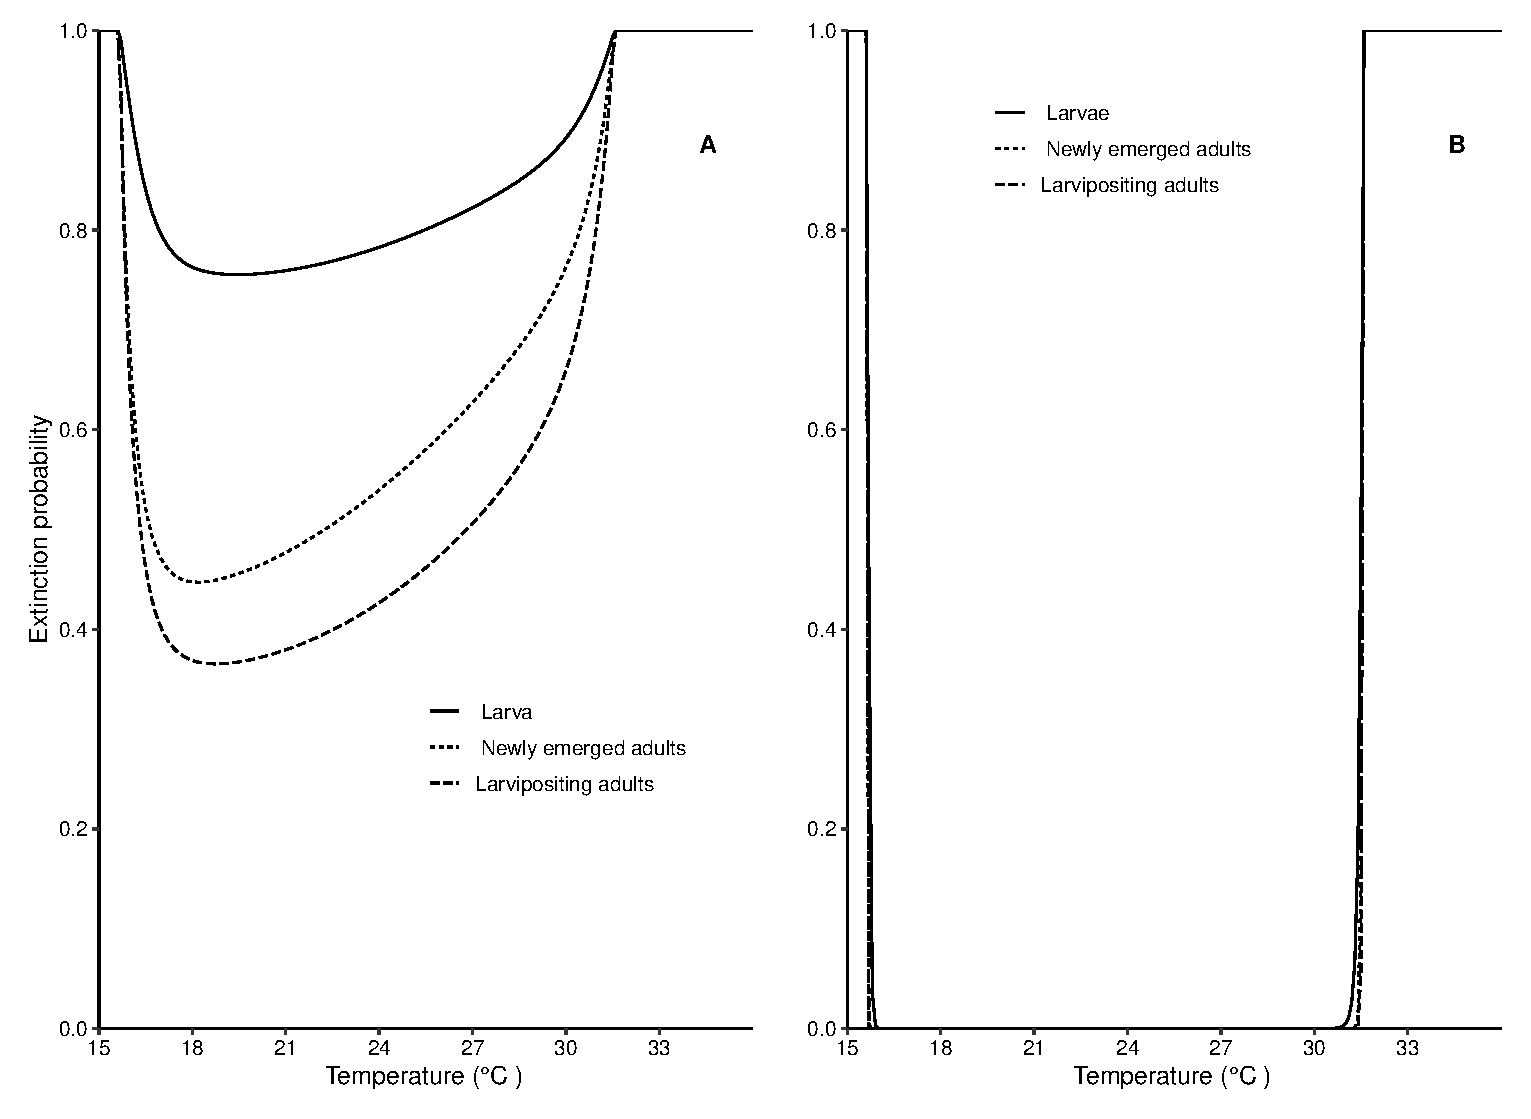
\includegraphics[width=0.75\textwidth]{Nov26-1.eps}
	% figure caption is below the figure
	\caption{{\bf Extinction probability as a function of temperature (15\degree C - 33\degree C) for different counting points}. (A) When pioneer populations consist of  a single larva, or newly emerged adult, or larval positing adult, respectively. (B) When pioneer population consist of  $100$, larvae, or newly emerged adult females, or larval positing adult females, respectively.}
	\label{fig:2}       % Give a unique label
\end{figure*}
%
\newpage

 If we assume a fixed temperature of 24\degree C, and simulate extinction probabilities  as a function of the daily mortality rates for female pupae (for the three counting points) starting with different initial population sizes. Extinction probabilities increase, and approach 1, as the daily mortality rates for female pupae increases. This is true for the three counting points. When daily mortality rate is $\geq$ 3.1\% per day, extinction probability is 1 for the three counting points (Fig \ref{fig:3}B).   



\begin{figure*}[h]
	% Use the relevant command to insert your figure file.
	% For example, with the graphicx package use
	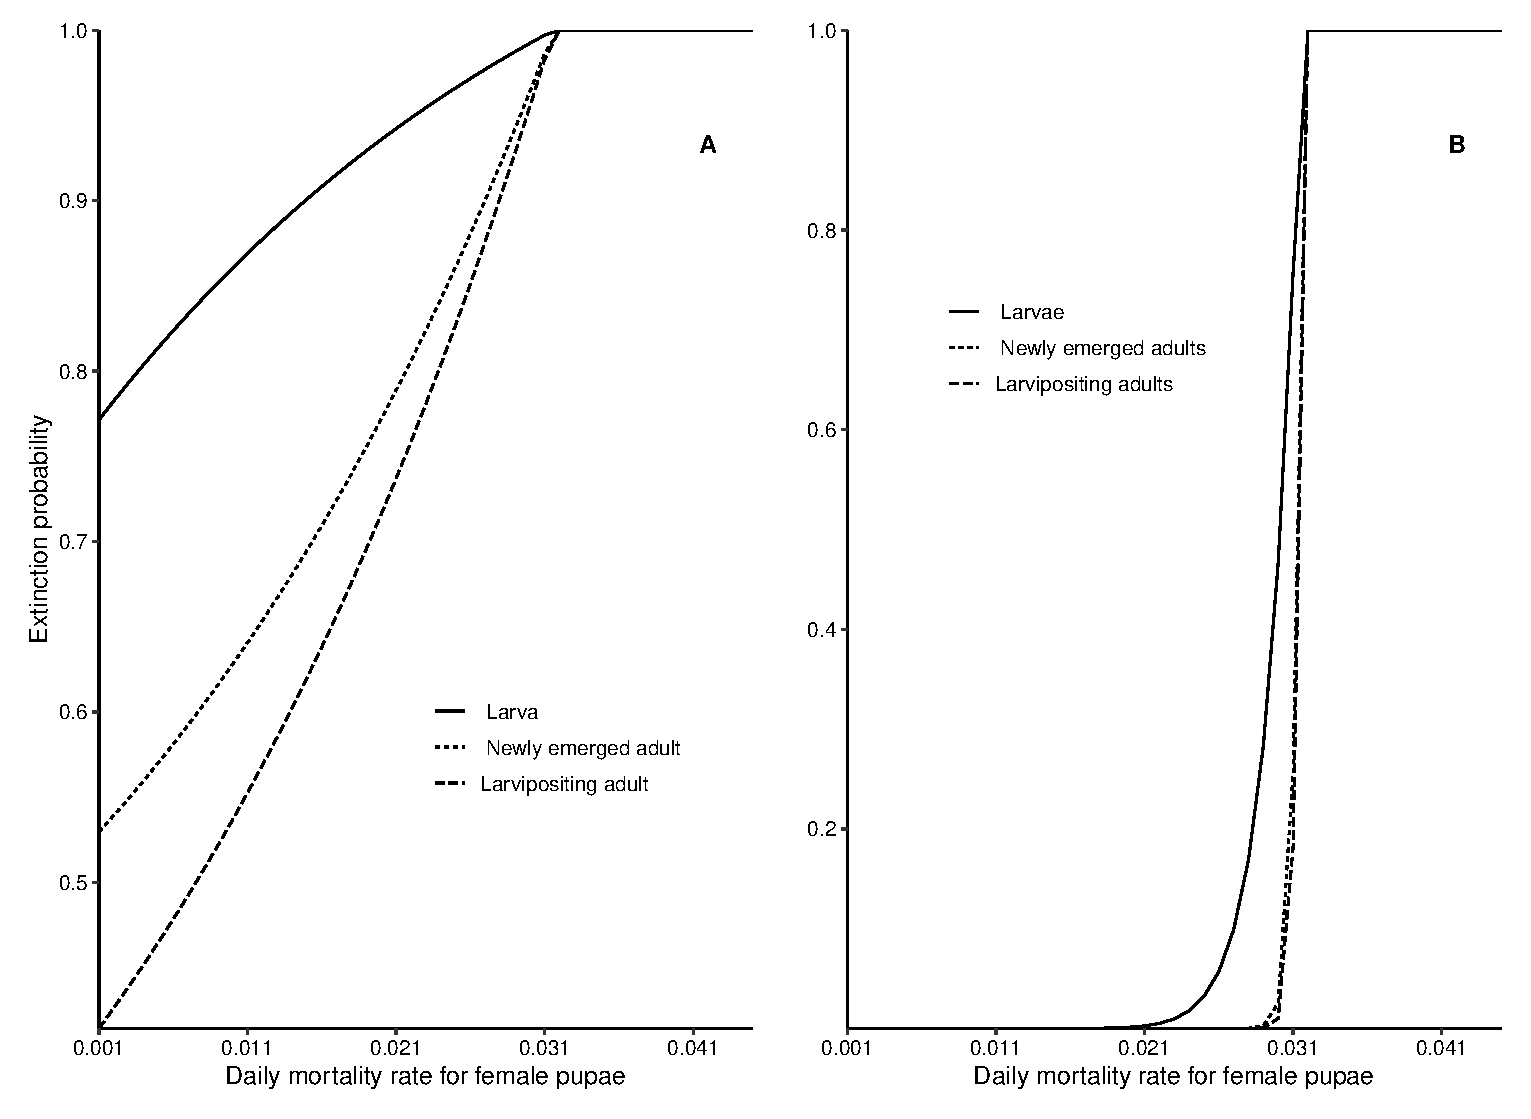
\includegraphics[width=0.75\textwidth]{demoOct102.eps}
	% figure caption is below the figure
		\caption{{\bf Extinction probability as a function of daily mortality rates for female pupae, at 24\degree C, for different count points}. (A) Each line represents extinction probabilities for a single larva, or newly emerged adult or larvipositing adult, respectively, in the initial populations (B) When pioneer populations consist of  $100$ larvae,  or newly emerged adults, or larvipositing adults, respectively.}
	\label{fig:3}       % Give a unique label
\end{figure*}
%

We present extinction probabilities as a function of the daily mortality rates for newly emerged adults. Extinction probabilities increase, for the three counting points, as the daily mortality rate for newly emerged adults increases. When the size of the initial population is increased to 100, for all counting points, extinction probability is 0 for daily mortality rates below 12\% per day. Extinction probability rapidly goes to 1, for all counting points, as daily mortality rate for newly emerged adults is $\geq$ 15.1\% per day (Fig \ref{fig:4}).
   


\begin{figure*}[h]
	% Use the relevant command to insert your figure file.
	% For example, with the graphicx package use
	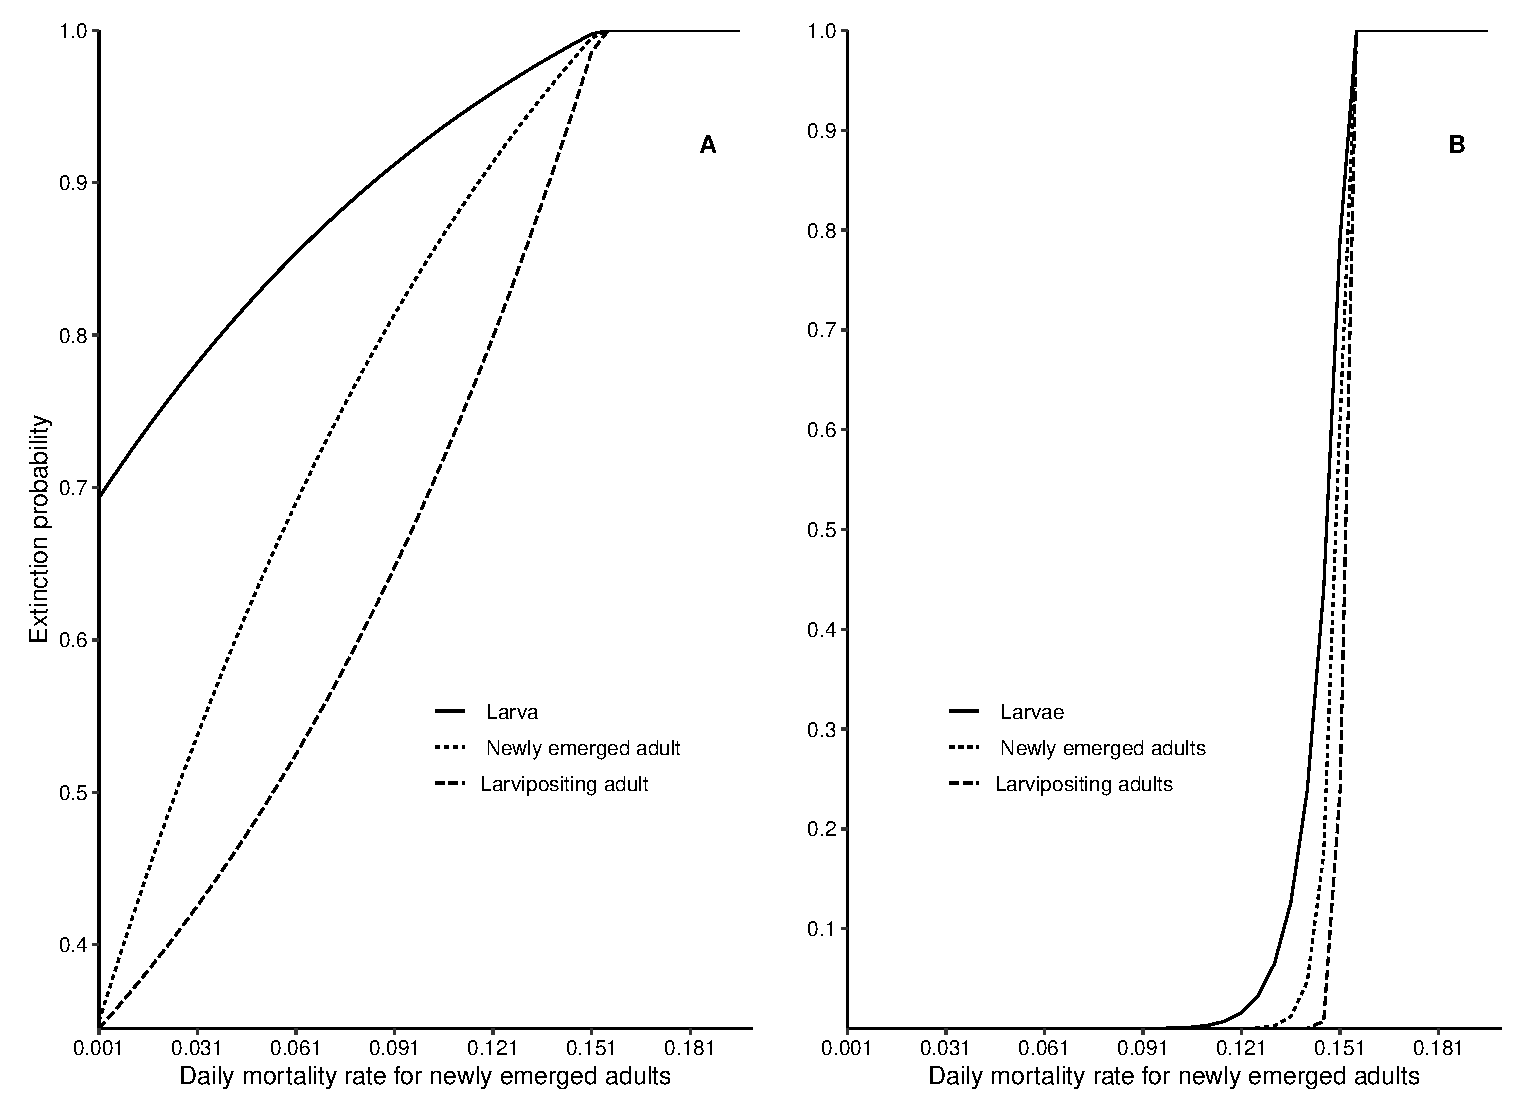
\includegraphics[width=0.75\textwidth]{demoOct103.eps}
	% figure caption is below the figure
	\caption{{\bf Extinction probability as a function of daily mortality rates for newly emerged adults at 24\degree C, for different count points}. (A) Each line represent extinction probabilities for a single larva, or  newly emerged adult or larvipositing adult, respectively,  in the initial populations (B) When pioneer populations consist of  $100$ larvae,  or newly emerged adults, or larval positing adults, respectively.}
	\label{fig:4}       % Give a unique label
\end{figure*}
%

\newpage

Extinction probabilities are ploted as a function of daily mortality rate for larvipositing adult females, for different counting points. There is a marked difference in extinction probabilities when the starting populations consist of a single larva, newly emerged adult and larvipositing adult, respectively. However, when the initial population is increased to 100, extinction probabilities go to 1, rapidly, for all counting points, when the daily mortality rate $\geq$ 3\% per day for larvipositing adults (Fig \ref{fig:5}). 



 \begin{figure*}[h]
 	% Use the relevant command to insert your figure file.
 	% For example, with the graphicx package use
 	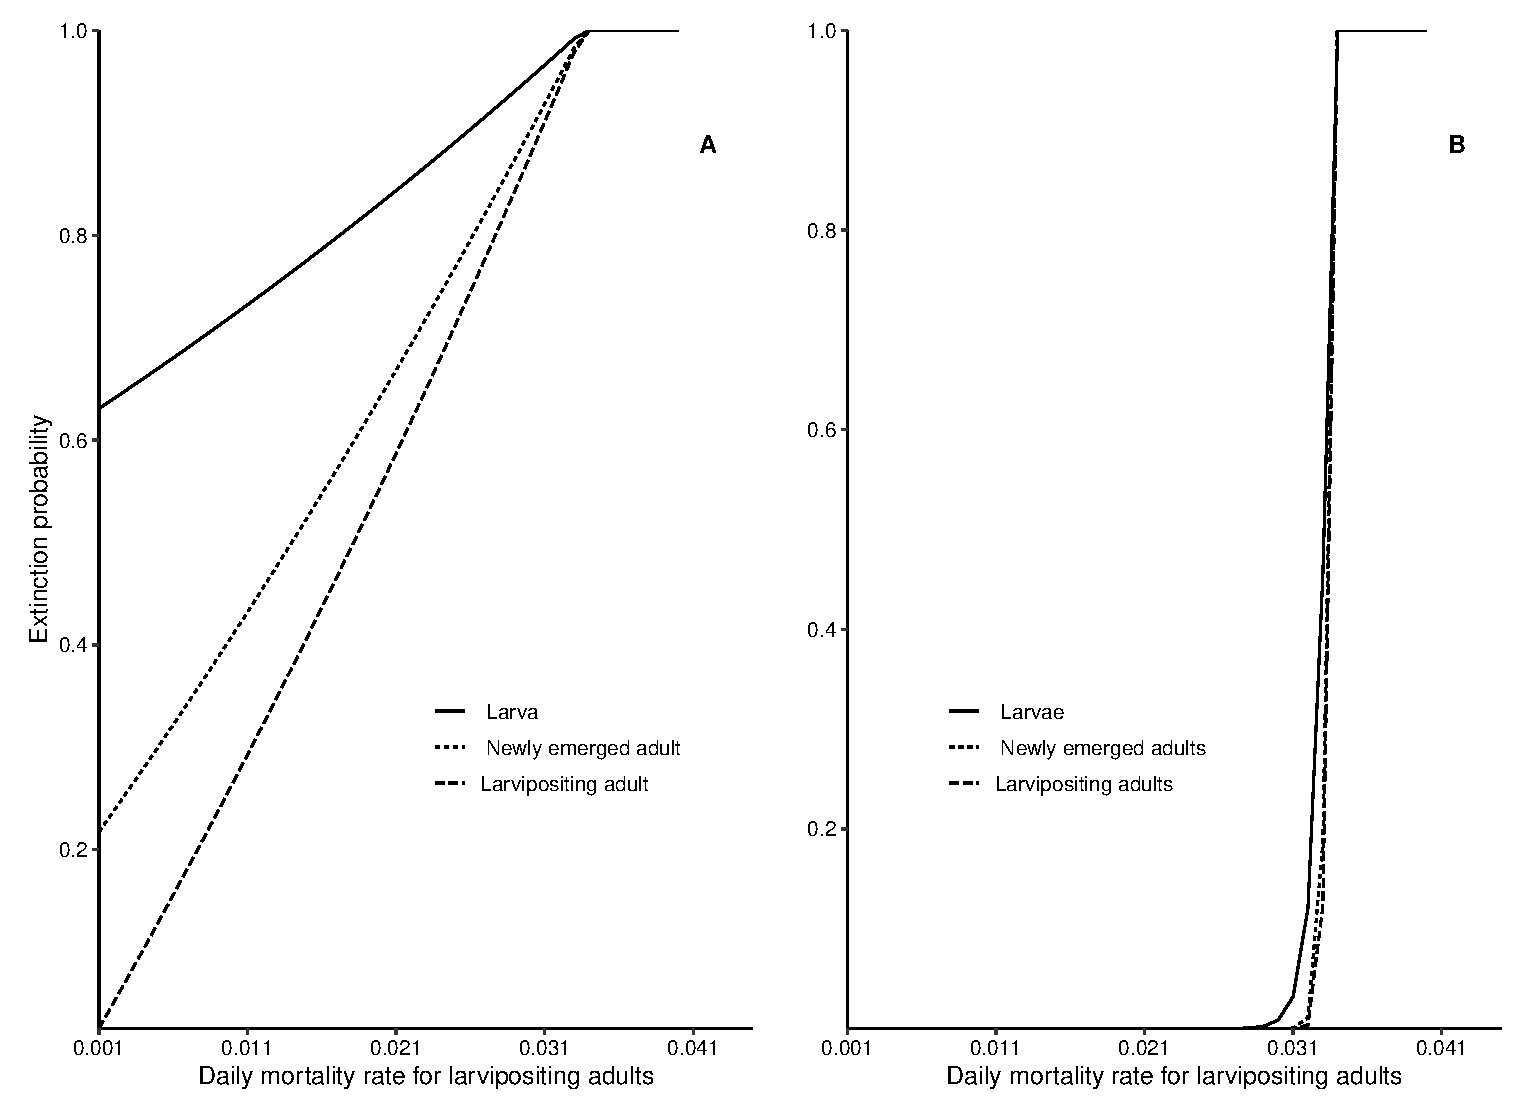
\includegraphics[width=0.75\textwidth]{demoOct1004.eps}
 	% figure caption is below the figure
 	\caption{{\bf Extinction probability as a function of temperature and daily mortality rates for larvipositing female adults at 24\degree C, for different count points}. (A) Each line represent extinction probabilities for a single larva, or  newly emerged adult or larvipositing adult, respectively, in the initial population (B) When pioneer populations consist of  $100$ larvae,  or  newly emerged adults, or larvaipositing adults, respectively.}
 	\label{fig:5}       % Give a unique label
 \end{figure*}
 %
 
When we increase the starting population to 500, for all counting points, extinction probabilities stays at 0 for all values of the daily mortality rate for adult females which are less than 3\% per day, daily mortality rates for newly emerged adults that are less than 15.1\% per-day and daily pupal mortality rates that are less than 3.1\% per-day. Moreover, when the daily mortality rate for larviposing female reaches 3.1\% per day, daily mortality rate for newly emerged adults exceeds 15.1\% per-day and daily mortality rate for female pupae exceeds 3.1\% per-day, extinction probability rapidly goes to 1. 
\newpage

\section{Discussion}

The life cycles of holometabolous insects, such as tsetse, is divided into four distinct stages, egg, larva, pupa and adult – each with distinct physiological features, and with differing responses to various environmental factors. In tsetse, for example,  the survival probability is high in the egg and larval stages, which are retained in the mother’s uterus \cite{Hargrove1999a}. Similarly, the pupa – which spends its life underground – often suffers low mortality, except at extremes of temperature \cite{PhelpsR.J.&Burrows}, although it may also be subject to density-dependent losses \cite{Rogers1984,RogersD.J.Randolph1984}. Mature female adults, too, exhibit low mortality \cite{Hargrove2011}: it is only the newly emerged, teneral adult that exhibits high mortality rates and which appear particularly susceptible to high temperatures \cite{Ackley2017a}. In this study, we investigate whether counting different stages influences our estimates of insect population persistence and basic reproduction number. We developed different models for each counting point, and analysed extinction probabilities and the basic reproduction number for the different life stages. We compared extinction probabilities for all starting points and derived a relationship between them. We developed a general model, for tsetse populations, that works for all counting points. \\



We demonstrated that the our estimate of the basic reproduction number was independent of our choice of the stage we counted. It does not matter whether we start with larvae, newly emerged adults or larvipositing adults, the average number of offspring an individual female is expected to produce remains the same. On the other hand, the estimated extinction probability is different for each counting stages. If the initial population consists of a single larva, extinction probability is higher than when the initial population consists of individuals that are either newly emerged or larvipositing adults. As indicated above, each stage of the tsetse life cycle typically experiences different mortalities \cite{Hargrove2005a}. The newly emerged adults, for instance, have higher mortality rates than the larvipositing adults  \cite{Hargrove2019a}. Even though the basic reproduction number does not depend on the stage that we count, a population which starts with larvipositing adults will have a higher chance of escaping extinction than a population which consists of larvae or newly emerged adults in its initial population. Notice, however, that this effect is only well marked when the size of the initial population is low. When the number of larvae, or newly emerged adults in the initial population is large, say $>$ 500, then it does not matter which stage we chose to count, the probability of extinction remains the same for all stages.\\

We calculated extinction probabilities as a function of fixed temperatures between 15\degree C and 35 \degree C for different counting points. The results agree with previous findings on temperature survival limits for tsetse population \cite{Edney1962,Kleynhans2011e,Pagabeleguem2016f,Are2019}. No tsetse population, regardless of the counting stage, can survive temperatures $<$ 16\degree C or $>$ 31\degree C, if exposed to these temperatures for a long period. When the initial population consists of a single individual, extinction probability did not drop below 0.3, regardless of the counting stage, even at optimal temperatures. When the initial population consists of a large population, extinction probability is zero for all temperatures within the limits 16 \degree C - 31 \degree  C, for all counting points (Fig \ref{fig:2}). The larger the size of the initial population the greater the chance of survival of tsetse populations. Tsetse populations can escape extinction at temperatures close to the lower and upper survival bounds, provided the initial population size is large (Figs \ref{fig:2}-\ref{fig:5}).\\


We set the temperature to 25 \degree C, which is the ideal temperature for optimal growth in tsetse population
\cite{Pagabeleguem2016f,Are2019}, and estimated extinction probability as a function of daily mortality rates for female pupae. For a population consisting of a single larva, extinction probability is high, at 0.78, even at low daily mortality rates for female pupae (0.1\% per-day). A population starting with a single larva is likely to go extinct even if the pupa is kept at optimal temperatures. A population starting with a single larvipositing adult has the highest chance of escaping extinction compared to other counting stages. As the daily mortality rates increases to 3.1\% per day, extinction probability goes to 1 in all cases. Moreover, when the size of the initial population is increased to 100 for each counting stage, the population will not go extinct for daily mortality rates for adult pupae that do not exceed 2.1\% per-day. At 25 \degree C, no tsetse population can survive if subject to a pupae daily mortality rate of 3.1\%. \cite{Hargrove2019a}. \\ 


We obtained extinction probabilities as a function of daily mortality rates for newly emerged adults, by
fixing the temperature at 25 \degree C. This allows us to assess the mortality in newly emerged adults that will be sufficient to drive tsetse populations to extinction, when all other factors are kept at optimal levels. When daily mortality for newly emerged adults is 0.1\% per-day, extinction probability, for a population starting with a single larva is 0.7. When the population starts with a single newly emerged adult, or a larvipositing female, the extinction probability is 0.35 when for the same daily mortality rates (0.1\% per-day) among  newly emerged adults (Fig \ref{fig:4} A and B). Any population starting with a single individual in any of the counting stages, will be go extinct when daily mortality rates in newly emerged adults are as high as 15\% per-day. As the sizes of the initial population increase to 100 each, extinction probability stays at zero for daily mortality rates, for newly emerged adults, below 12\% per-day. Substantially high levels of mortality are thus required to achieve extinction if mortality is increased only in newly emerged adults.
 

Control techniques that are presently being used for increasing tsetse mortalities (such as tiny targets etc \cite{Hargrove2000,Esterhuizen2006,Shaw2015,Mbewe2018a}) are more likely to kill larvipositng adults than imature adults. Newly emerged adults have poorly developed thoracic musculature and low fat reserves, these two factors may limit thier ability to fly long distances for them to be caught in stationary traps. Mobile baites such as insecticide treated cattles on the other hand, tends to be more effective in catching newly imerged adults than the stationary targets \cite{Hargrove1991}. Hargrove et al \cite{HargroveJ.W.HollowayM.T.P.ValeG.A.GoughA.J.E.Hall1995} carried out a large scale experiment that used  odour baited traps to sample  {\it Glossina m. morsitans} Westwood and {\it G.pallidipes} Austen in Zimbawe. For both species, very small numbers of newly emerged flies compared to larvipositing adults were caught. The level of daily mortality that is required for elimination of a closed population of tsetse can be safely taken as 3.5\% per-day (daily mortality rates in larvipositing adults that will achieve elimination) (Fig \ref{fig:4} A and B).  \\


We calculated extinction probabilities as a function of daily mortality rates for larvipositing female adults by keeping the temperature at 25 \degree C. When the pioneer populations consist of single individuals of the three stages, and the daily mortality rate for larvipositing females is increased from 0.1\% per-day to 3\% per-day, extinction probabilities go to one at different rates, for different counting points. No tsetse population can avoid extinction if the daily mortality rate for larvipositing females exceeds 3.1\% per-day\cite{Are2019}.




 



\section{Conclusion}

The general model works for all counting points, for different decomposition of the recruitment rates between the life stages. We showed that extinction probability for different counting stages depends on the probability of recruitment between these stages. We showed that previous models used to estimate extinction probability for tsetse populations are special cases of the general model. \\

We can predict insect population persistence only if we count and calculate carefully, taking account of different stages. We caution that the basic reproduction number is not sufficient to accurately determine insect population persistence. Our results offer insights into population dynamics and provide tools that will help with more detailed models of insect populations. Finally, we advise that demographic studies of insects should be clear about life stages and counting points.\\

A limitation of the present study is that we do not consider density dependencies in the population. We are assuming situations were populations are below their carrying capacities. Our results show that when the population is large enough to consider density dependent effects, the counting points may not matter.





%\begin{acknowledgements}
%If you'd like to thank anyone, place your comments here
%and remove the percent signs.
%\end{acknowledgements}


% Authors must disclose all relationships or interests that 
% could have direct or potential influence or impart bias on 
% the work: 
%
 \section*{Conflict of interest}
%
 The authors declare that they have no conflict of interest.


% BibTeX users please use one of
%\bibliographystyle{spbasic}      % basic style, author-year citations
%\bibliographystyle{spmpsci}      % mathematics and physical sciences
%\bibliographystyle{spphys}       % APS-like style for physics
\bibliographystyle{ieeetr}
\nocite{*}
\bibliography{mybibloInsectdemo}   % name your BibTeX data base
%\printbibliography
% Non-BibTeX users please use
%\begin{thebibliography}{}
%
% and use \bibitem to create references. Consult the Instructions
% for authors for reference list style.
%
%\bibitem{RefJ}
%% Format for Journal Reference
%Author, Article title, Journal, Volume, page numbers (year)
% Format for books
%\bibitem{RefB}
%Author, Book title, page numbers. Publisher, place (year)
% etc
%\end{thebibliography}

\end{document}
% end of file template.tex

